\section{Results}
\subsection{Study 1: when models choose}
At high, pooled over the four models, the share of calls with reported reasoning was \bHone{} percentage points higher on traps than on controls (95\% interval \bHoneLo{} to \bHoneHi{}).
Per-model rows are in \url{paper/generated/crt-b-h1.tex}.
By the pre-specified rule this supports edit sensitivity.
Whether the effect exceeds 10 points is unresolved, because the interval spans it.
We had predicted a null or small effect.
GPT-5.6 Luna (\bHoneLunaFive{}), GPT-5.6 Terra (\bHoneTerra{}) and Sonnet 4.6 (\bHoneSonnet{}) met the support rule on their own, and GPT-6 Luna (\bHoneLunaSix{}, \bHoneLunaSixLo{} to \bHoneLunaSixHi{}) met none of the three rules.

\begin{figure}[!tbp]
\centering
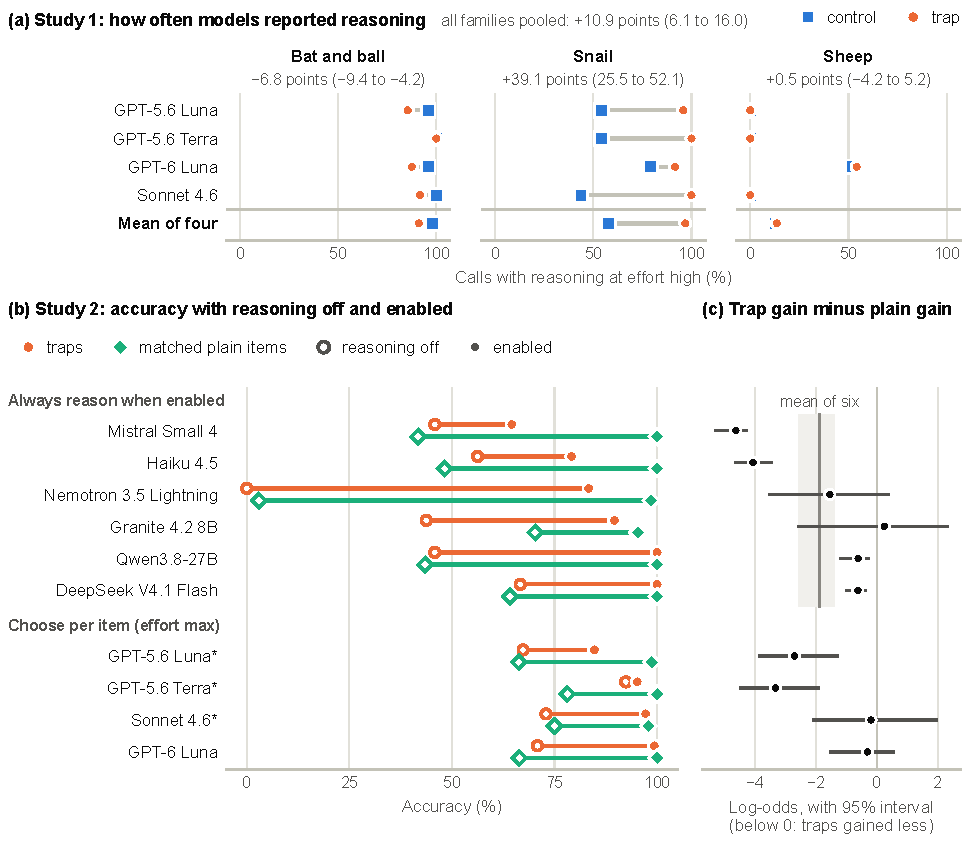
\includegraphics[width=\textwidth]{fig-results}
\caption{Main results of both studies.
(a) Study 1: the share of calls at effort high on which each model reported reasoning, on control and trap items of each family.
The line under each family name gives the post hoc trap minus control difference in percentage points, pooled over the four models, with its pointwise 95\% interval.
The heading gives the pre-specified primary contrast, \bHone{} points (95\% interval \bHoneLo{} to \bHoneHi{}).
(b) Study 2: accuracy with reasoning off (open markers) and enabled (filled markers), on traps and on plain items reweighted to match the traps' off accuracy on the first off draw.
The open plain markers show the second off draw, on which the matched gain is computed, so they can sit away from the trap marker.
An asterisk marks models for which enabled does not mean forced.
(c) The trap gain minus the matched plain gain in log-odds, with 95\% bootstrap intervals.
The band is the mean over the six models that always reason, \aAone{} (\aAoneLo{} to \aAoneHi{}).
Qwen and DeepSeek reach 100\% with reasoning enabled on both item types, so their differences depend on the bound applied to accuracy.}
\label{fig:results}
\end{figure}

The family breakdown is post hoc (Figure~\ref{fig:results}a).
Pooled over the four models, the difference was \bFamSnail{} points on snail (\bFamSnailLo{} to \bFamSnailHi{}), \bFamBatball{} on bat and ball (\bFamBatballLo{} to \bFamBatballHi{}) and \bFamSheep{} on sheep (\bFamSheepLo{} to \bFamSheepHi{}).
On bat and ball, models reasoned slightly more often on the two-step control than on the trap.
On sheep, GPT-5.6 Luna, GPT-5.6 Terra and Sonnet 4.6 reported no reasoning on any observed call, while GPT-6 Luna reasoned on about half of both versions.

Reasoning tracked need only weakly, with slopes of an item's reasoning rate at high on the estimated benefit of max effort of \bSlopeLunaFive{} for GPT-5.6 Luna, \bSlopeTerra{} for Terra, \bSlopeLunaSix{} for GPT-6 Luna and \bSlopeSonnet{} for Sonnet 4.6.
Most errors at high fell on calls without reported reasoning (Figure~\ref{fig:graph-b-errors}).
That was \bSkipWrongLunaFive{} of \bWrongLunaFive{} for GPT-5.6 Luna, \bSkipWrongLunaSix{} of \bWrongLunaSix{} for GPT-6 Luna and \bSkipWrongSonnet{} of \bWrongSonnet{} for Sonnet 4.6, and GPT-5.6 Terra made only \bWrongTerra{} errors.
The models chose which calls to reason on, so this shows where errors fell, not what reasoning would have fixed.
Of GPT-5.6 Luna's \bWrongLunaFive{} errors, \bSheepAllWrongLunaFive{} were on sheep traps.

\begin{figure}[tbp]
\centering
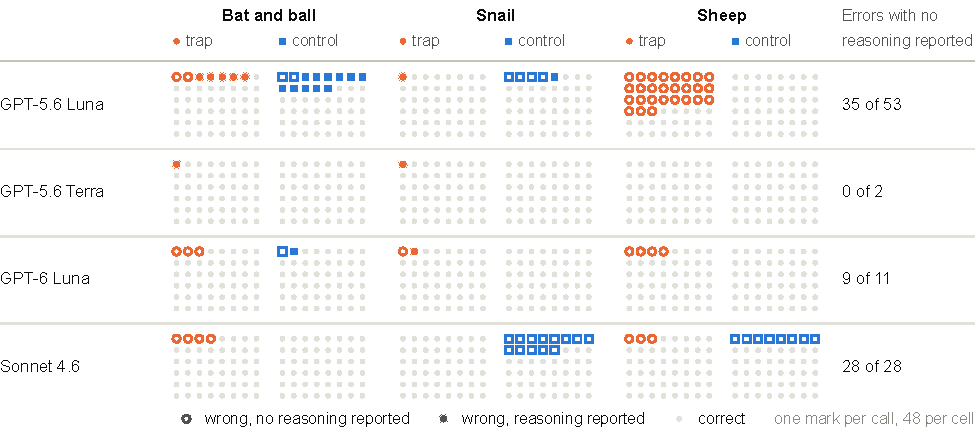
\includegraphics[width=\textwidth]{fig-graph-b-errors}
\caption{Where the wrong answers fell at effort high in Study 1.
Each mark is one completed call from the primary arm of a model that chooses whether to reason.
Each cell holds one model's calls on the traps (circles) or controls (squares) of one family, both wordings pooled.
Wrong answers are coloured, with an open mark when the call reported no reasoning and a filled mark when it did.
Grey marks are correct answers, with or without reasoning.
Marks are sorted within a cell, so position carries no item information.
The right column counts wrong answers without reasoning among all wrong answers of that model.}
\label{fig:graph-b-errors}
\end{figure}

\subsection{Study 2: with reasoning enabled}
Every model's trap gain was positive, but no model passed the rule for a larger trap gain than matched plain gain (Figure~\ref{fig:results}c; \url{paper/generated/crt-a-a1.tex}).
Six model intervals lay below zero and four spanned it.
The mean over the six always-reasoning models was \aAone{} log-odds (\aAoneLo{} to \aAoneHi{}), and \aAoneNoSheep{} (\aAoneNoSheepLo{} to \aAoneNoSheepHi{}) without sheep.
With one common bound ($n=48$) for every cell, the six-model mean becomes \aAoneCommonMean{}, a sensitivity check outside the plan.

With reasoning enabled every model scored at least \aPlainOnMin{}\% on the plain set, above the best model with reasoning off (\aPlainOffMax{}\%).
The planned comparison of a strong model off with a weak model on therefore had no overlap, and whether reasoning helps on traps beyond general capability could not be evaluated.
A harder plain set (3 to 16 operations) did not close the gap in a pilot, where the weakest enabled models scored \aPilotOnMin{}\% and GPT-5.6 Terra with reasoning off \aPilotTerraOff{}\%.

For the six always-reasoning models, method answers fell from \aMethodPerCallOff{}\% of trap calls with reasoning off to \aMethodPerCallOn{}\% enabled, while other wrong answers nearly disappeared.
Most remaining wrong trap answers were therefore method answers, \aOnMethodSix{} of \aOnWrongSix{} enabled errors (Figure~\ref{fig:graph-a-errors}).
For Mistral and Granite, method answers became more frequent per trap call when reasoning was enabled.
Visible steps with reasoning off came close to or above hidden reasoning on traps for Granite, Haiku and Mistral, and below it for Nemotron, Qwen and DeepSeek (\url{paper/generated/crt-a-a4.tex}).

\begin{figure}[tbp]
\centering
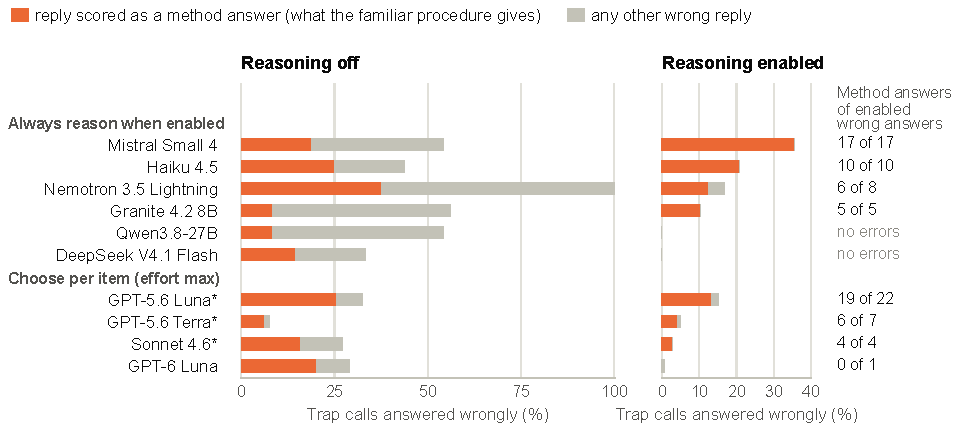
\includegraphics[width=\textwidth]{fig-graph-a-errors}
\caption{Wrong answers on trap items in Study 2, as a share of completed trap calls, with reasoning off and enabled.
Orange marks method answers, grey any other wrong reply, unparsed replies included.
Both panels use the same distance per percentage point.
The right column gives each model's method answers among its wrong answers with reasoning enabled.
Pooled over all ten models, \aOnMethod{} of \aOnWrong{} enabled errors were method answers.
For the choosers, enabled means effort max, and an asterisk marks models that did not always reason there.}
\label{fig:graph-a-errors}
\end{figure}
